\documentclass[a4paper,12pt,numbers=noenddot]{report}

\usepackage{polski}
\usepackage[utf8]{inputenc}
\usepackage{graphicx}
\usepackage{cite}
\usepackage{float}
\usepackage{url} 
\usepackage{hyperref}
\usepackage{amsmath}
\usepackage{gensymb}
\usepackage{pdfpages}
\usepackage[nottoc,numbib]{tocbibind}
\usepackage{etoolbox}
\usepackage{enumitem}

\usepackage{titlesec, blindtext, color}

\titleformat{\chapter}[hang]{\Huge\bfseries}{\thechapter{. }}{0pt}{\Huge\bfseries}


\usepackage[
  inner = 3cm,
  outer = 2.5cm,
  top = 2.5cm,
  bottom = 2.5cm,
]{geometry}


\title{TYTUŁ pracy}
\date{\today}
\author{Hubert Marcinkowski}

\begin{document}
	\nocite{*}
	\pagenumbering{gobble}
	%\maketitle
	
\includepdf{first_page.pdf}

	\newpage
	\pagenumbering{arabic}
	\tableofcontents
	\newpage
	%\setcitestyle{square}	
%CHAPTER_______________________________________________________________________________________WSTĘP_______	
\chapter{Wstęp}
Projektowanie interfejsów jest tematyką bardzo złożoną i nadzwyczaj kluczową w procesie tworzenia aplikacji, w tym, między innymi, gier komputerowych. Złe zaprojektowanie tej części w prosty sposób może przyczynić się do całkowitego braku zrozumienia całego przesłania gry przez użytkowników. Istnieje wiele metodologii mających na celu analizę jakości stworzonego projektu - od metod całkowicie subiektywnych po takie, które stawiają za zadanie sprowadzenie jak największej części elementów do postaci parametrycznej. 

- Trudne zadanie związane z tym, że poszukiwany jest pewien zbiór reguł, który ułatwiłby proces projektowania. 
- Część z przedstawianych rozwiązań wybitnie nie pasuje do dziedziny mobilek
- Problemy związane z projektowaniem dla mobilek
- Przygotowane zostały heurystyki, które mają na celu dokładne określenie jakie warunki aplikacja musi spełniać, by mogła zostać dobrze odebrana przez użytkowników
- coś o tym, że użytkownik w czasie gry często zostaje postawiony przed przyswojeniem bardzo abstrakcyjnego zadania w celu zrozumienia, a co za tym idzie grania w daną grę

W pracy tej opisane zostało badanie mające na celu zweryfikowanie wpływ spełniania tych heurystyk na pozna
%CHAPTER__________________________________________________________________________CEL, ZAŁOŻENIA, ZAKRES__
\chapter{Cel, założenia oraz zakres pracy}
Celem tej pracy było zbadanie wpływu określonych heurystyk dotyczących projektowania interfejsów na jakość przyswajania nowych mechanik gry mobilnej, która z nich korzysta. Badaniu podane zostały zasady, które odnoszą się do użyteczności tworzonych aplikacji.

Ustalanie heurystyk ma na celu określenie wytycznych, za pomocą których deweloperzy gier są już w stanie określić, czy przygotowywany przez nich projekt ma szansę spodobać się odbiorcom. Spodziewać się można, że przy porównaniu dwóch aplikacji zajmujących się jednym zagadnieniem, gdzie jedna z nich spełnia większą ilość heurystyk użyteczności z zadanego zakresu to poprawnie wykonane testy wykażą, że jest ona bardziej użyteczna. Cecha ta definiuje między innymi stopień wydajności z jaką użytkownik jest w stanie zrozumieć prezentowane mu przez aplikację treści. Oznaczać to może, że badając, jakie heurystyki spełnia dana gra, jesteśmy w stanie oszacować jak zrozumiała mogła by ona być dla jej docelowego użytkownika.\\
Bazując na tych założeniach, praca ta ma na celu sprawdzenie następujących hipotez:

\begin{enumerate}
\item Zrozumienie mechanik gry mobilnej przychodzi użytkownikom łatwiej dla gier spełniających więcej heurystyk użyteczności.
\item Użytkownicy popełniają mniej błędów w wypadku gier spełniających więcej heurystyk użyteczności
\item Użytkownicy grający w grę spełniającą mniej heurystyk użyteczności osiągają gorsze wyniki od tych, którzy grają w wersję spełniającą ich więcej.
\end{enumerate}

W celu ich przetestowania przeprowadzone zostało doświadczenie, w którym za pomocą testów rozgrywki (ang. \textit{playtesting}) badane były cztery wersje tej samej gry mobilnej w różnym stopniu spełniające wybrane heurystyki odnoszące się do użyteczności gier. Dane z każdego testu były zapisywane automatycznie przez aplikację do pliku a następnie zostały one przeniesione do arkusza kalkulacyjnego, gdzie wykonano ich analizę. Wyniki opracowano i przedstawiono w postaci czytelnych dla osób postronnych wykresów.


%CHAPTER_______________________________________________________________________________WYJAŚNIANIE POJĘĆ___
\chapter{Grywalność w grach mobilnych}
Przed rozpoczęciem analizy kluczowym zdaje się dokładne wyjaśnienie podstawowych pojęć, jakie wykorzystywane są w tej pracy. W tym rozdziale wyjaśnione zostanie co definiowane jest jako mechanika gry, doświadczenie użytkownika, czym jest grywalność i użyteczność a także przybliżone będą ograniczenia i przeszkody związane z rozgrywką na urządzeniach mobilnych.

\section{Heurystyka}
Mianem heurystyk określa się zestaw zasad, których przeznaczeniem jest zwiększenie prawdopodobieństwo rozwiązania określonego problemu \cite{art_WithHeuristic}. Służą one jako pomoc przy rozwiązywaniu problemów przy pomocy eksperymentalnych metod. W przypadku metod mierzących użyteczność skupiają się one na zagadnieniach, które sprawiają problemy podczas interakcji\cite{art_Nielsen}\cite{art_evaluatingPlayabilityMG}. 

\section{Mechanika gry}
Mechaniki gry zdefiniować można jako zestaw reguł zaprojektowanych w celu zapewnienia użytkownikowi interakcji ze stanem gry. Zestawienie różnych mechanik rozgrywki określa stopień skomplikowania jak również ilość akcji, których wykonanie wymagane jest od użytkownika. Innymi słowy określić je można jako zbiór zasad, które pozwalają graczowi na postęp w przestrzeni gry. \cite{online_GameMechanics}

\section{Doświadczenie użytkownika}

Pojęciem doświadczenia użytkownika (\textit{User Experience} - UX) opisuje się całość wrażeń, z którymi spotyka się osoba podczas procesu użytkowania określonego produktu bądź usługi. Pod tym pojęciem zawierają się wszelkie aspekty interakcji człowiek-komputer oraz wrażenia osoby użytkującej dotyczące takich aspektów systemu jak na przykład łatwość w użyciu czy wydajność. Wyróżnia się trzy czynniki wpływające na UX: system, użytkownik oraz kontekst użycia. \cite{online_UXDef}
Celem projektowania dobrego UX jest osiągnięcie jak największej produktywności przy pracy z systemem, czyli innymi słowy - spełnienie oczekiwań użytkownika. Ważnym aspektem poprawnie zaprojektowanego UX jest również to, by korzystanie z przygotowanego systemu było przyjemne i proste. Projektowania doświadczenia użytkownika się między innymi w celu wyeliminowania błędów interfejsów, czy zmniejszenia ilości operacji, które wymagane są do wykonania określonego zadania.
\cite{art_UserExperience}

\section{Użyteczność}
Użyteczność definiowana jest jako podatność danej aplikacji do bycia używaną przez ludzi prosto i wydajnie\cite{art_Usability}. Jest to swojego rodzaju miara pozwalająca na określenie stopnia, w jakim dany produkt może być zrozumiany i wykorzystywany. Określa ona również jak bardzo aplikacja jest zachęcająca dla użytkowników, którzy jej używają w określonym środowisku. \cite{art_evaluationOfMGevaluationSystem} 
\\
Można wyróżnić siedem podstawowych czynników użyteczności: \cite{art_UsabilityEvaluationSystematicReview}
\begin{enumerate}
\item Bezmyślność (ang. \textit{learnability}) - określa jak łatwo użytkownik jest w stanie wykonać postawione mu przez grę zadanie za pierwszym podejściem oraz jak szybko jest w stanie polepszyć uzyskany wynik.
\item Wydajność (ang. \textit{efficiency}) - definiuje czas, jaki potrzebny jest doświadczonemu użytkownikowi na wykonanie zadania.
\item Zapamiętywanie (ang. \textit{memorability}) - miara oznaczająca łatwość, z jaką użytkownik potrafi wrócić do gry po pewnej przerwie.
\item Błędy (ang. \textit{errors}) - ilość błędów gry, jakie użytkownik popełnia w trakcie rozgrywki.
\item Satysfakcja użytkownika (ang. \textit{user satisfaction}) - określa nastawienie użytkownika do gry
\item Prostota (ang. \textit{simplicity}) - stopień swobody z jakim wykonywać można zadania w grze. Odnosi się zwykle do nawigacji w różnego rodzaju ekranach menu.
\item Czytelność (ang. \textit{readability}) - określa jak łatwo użytkownik jest w stanie zrozumieć zawartość gry.
\end{enumerate}

Wyróżnia się dwie główne metodologie mierzenia użyteczności: testowanie poprzez rozgrywkę (ang. \textit{play-testing}) oraz opinie ekspertów (ang. \textit{expert review}).

\subsection{Mierzenie użyteczności}
Testowanie poprzez rozgrywkę zakłada, iż testowanie odbywa się przez osoby z grupy docelowej tworzonego produktu\cite{art_evaluatingPlayabilityMG}. Wchodzą oni w interakcję z aplikacją a ich zachowanie i wrażenia z rozgrywki są zbierane przez samą grę lub przez obserwujących ich badaczy. Metoda ta pozwala na bezpośrednie zaobserwowanie przez deweloperów w jaki sposób gracze wykonują polecenia, które przekazywane im są za pośrednictwem aplikacji.
Zauważyć jednak należy wiele przeszkód, które nie pozwalają na określenie tego sposobu sprawdzania użyteczności jako bardzo przystępnego. Przygotowanie odpowiedniego środowiska do przeprowadzenia badania niejednokrotnie może wiązać się z dużymi nakładami pieniężnymi jak i czasowymi. Testowanie przez graczy spoza zespołu deweloperskiego nie pozwala na uzyskanie wymiernych wyników do czasu, aż dostępny jest działający prototyp aplikacji. Musi on zwykle być wycinkiem zawierającym wszelkie właściwości, którymi cechować się ma finalna wersja gry. Problem zwiększa się w przypadku, gdy podczas takich testów na jaw wychodzą błędy związane z grywalnością produktu. Próba ich naprawy nierzadko oznaczać może konieczność wprowadzenia poważnych zmian w projekcie, co z kolei prowadzi do poniesienia dużych kosztów przez deweloperów. Zignorowanie tych problemów również jest ryzykowne, gdyż istnieje szansa na to, iż mogą one wpłynąć negatywnie na wrażenia związane z rozgrywką \cite{art_evaluationOfMG}.

Z tego też powodu przez wielu badaczy testowanie za pomocą opinii ekspertów jest dużo bezpieczniejszym podejściem \cite{art_UsabilityTestingComp}. W tym wypadku rzadko zdarza się, by użytkownicy z grupy docelowej brali udział w badaniu. Testerami jest tu dwóch lub więcej ekspertów biegłych w dziedzinie użyteczności aplikacji \ref{art_Nielsen}. Zwykle zakresy ich ekspertyz są zbiorami jak najbardziej rozłącznymi tak, by uzyskać jak największy obszar oceny. Przeprowadzają oni niezależne testy w oparciu o ogólnie przyjęte heurystyki i następnie porównując swoje notatki podejmują finalną decyzję odnośnie danej aplikacji.
Dużą zaletą tej metody jest szybkość, z jaką otrzymać można pełną ocenę użyteczności gry. Eksperci dysponując dużym zakresem wiedzy w sprawdzanej dziedzinie są w stanie przeprowadzić pełną ewaluację w zaledwie kilka godzin używania zarówno funkcjonalnych prototypów jak i takich, które w małym stopniu odwzorowują finalny produkt (papierowe makiety, koncepty czy nawet same opisy interakcji). 

Wybór metody, którą należy obrać do analizy często zależne jest od czynników takich jak ilość czasu i pieniędzy, jakie można zainwestować w proces testowania użyteczności. W wypadku, gdy niedobór środków, które można na taką ocenę przeznaczyć jest czynnikiem pomijalnym najlepszym rozwiązaniem jest hybryda tych rodzajów badań. Pozwala to na połączenie ich zalet jednocześnie minimalizując ich wady.

\section{Grywalność}
Grywalność określić można jako zestaw własności, które opisują doświadczenie gracza (ang. \textit{Player Experience}) przy użyciu określonego systemu growego, którego głównym celem jest zapewnienie rozrywki poprzez jego użytkowanie zgodnie z jego przeznaczeniem. \cite{art_Playability} Odnosi się do jakości samej gry. Jest to pojęcie często używane zarówno w procesach projektowania jak i analizy gier pod względem ich reguł, mechanik czy zadań stawianych przez nie graczom. Na grywalność wpływa bardzo wiele czynników związanych z samą rozgrywką, jak na przykład responsywność na akcje gracza czy intensywność interakcji.
Grywalność składa się z trzech komponentów: podstawowych mechanik (zasady oraz zadania, które użytkownik ma wykonać), narracji oraz interaktywności (zestaw elementów, które są widoczne dla gracza i z którymi może wejść w interakcję w przestrzeni gry). \cite{art_UserExperience}

Jak można zauważyć, pojęcie grywalności jest ściśle powiązane z użytecznością. Zaznaczyć jednak należy, że w kontekście gier, jest ono dużo dokładniejsze. Mierzy ono nie tylko jak dobrze gracz jest w stanie wykonywać zadania, ale również to, czy odczuwa w trakcie wykonywania tych operacji przyjemność. Aspekty miary, jaką jest grywalność nie są ściśle określone dla każdej gry. Oznacza to, że w zależności od gatunku do jakiego przypisana jest dana aplikacja, przypisać można różne wagi poszczególnym jej aspektom.

Zarówno jak w przypadku użyteczności, wyróżnić można siedem czynników charakteryzujących grywalność:

\begin{enumerate}
\item Efektywność - czas i środki, jakie potrzebne są, by zaoferować graczom przyjemne doświadczenia z wykonywania zadań postawionych przez grę.
\item Bezmyślność (ang. \textit{learnability}) - stopień w jakim gracz jest w stanie zrozumieć i nauczyć się systemów i mechanik gry. Zauważyć należy, że w przypadku gier nie zawsze wskazane jest, by gracze zrozumieli wszystkie zasady w nich panujące. Niekiedy krzywa uczenia projektowana jest w taki sposób, by wymusić na graczu posiadanie zadanych umiejętności, by posunąć się dalej w rozgrywce.
\item Zanurzenie - określa w jakim stopniu zawartość danej gry jest wiarygodna do tego stopnia, że gracz bezpośrednio wczuwa się w wirtualny świat. Oznacza to, że podczas wykonywania wymaganych interakcji użytkownik czuje się częścią tego świata.
\item Satysfakcja - przyjemność pochodząca z grania w grę bądź wynikająca z jakiegoś określonego aspektu gry. Wyróżnić można tu zarówno zabawę, jaką odczuł użytkownik podczas rozgrywki, ale także zawód którego mógł doznać przy wykonywaniu wybranych zadań.
\item Motywacja - zestaw charakterystyk gry, który zachęca gracza do wykonywania określonych akcji i kontynuowania dalszej rozgrywki po ich wykonaniu. Zaliczać się do nich mogą chociażby nagrody w postaci zasób kluczowych dla danej gry, które wręczane są użytkownikowi po spełnieniu zadanego warunku.
\item Emocje - odnosi się do bezwarunkowych impulsów, jakie odczuwa gracz w odpowiedzi na stymulant w postaci gry.
\item Socjalizacja - zestaw parametrów gry, które zachęcają do współpracy, bądź interakcji między użytkownikami. Ten rodzaj wspólnych doświadczeń sprawia, iż dzięki relacjom, które nawiązywane są podczas grania, gracze doceniają grę w zupełnie innym wymiarze 
\end{enumerate}


%CHAPTER____________________________________________________________________________________STAN TECHNIKI__
\chapter{Stan techniki}
Gry komputerowe są bardzo charakterystyczną formą aplikacji. Wymagane od nich jest nie tylko to, żeby wykonywały jakieś zaprogramowane reakcje, czy obliczenia, ale także to, by gdy używane są przez grupę użytkowników docelowych w określonym środowisku było dobrą rozrywką. Duży nacisk przy produkcji stawiany jest zatem w poprawne ich zaprojektowanie. W dziedzinie projektowania trudno jednak stwierdzić, w którym momencie można zakończyć ten etap tworzenia produktu. 

\section{Dziesięć heurystyk Nielsena}
Poszukiwano zatem zestawu zasad, które spełnić powinna gra. Znalezienie takowych oznaczać by mogło, że dokładniejsze ich wypełnianie daje większe szanse na odniesienie sucesu. W 1990 roku Nielsen i Molich \cite{art_Nielsen} zaproponowali zestaw dziesięciu heurystyk, które powinny być spełniane przy projektowaniu interfejsu użytkownika. Zaliczały się w nich między innymi konieczność informowania odbiorcy o statusie systemu, czy niedopuszczanie do tego, by odbiorca mógł popełnić jakikolwiek błąd w procesie użytkowania aplikacji. Zasady te były rozwijane przez lata i przez wielu uważane są jako absolutna podstawa przy projektowaniu. 

\section{Heurystyki PLAY}
Projektowanie gier zakłada jednak czasem cele inne niż to, czy interfejs jest prosty w użyciu i czy udostępnia proste wykonywanie zadań, gdyż gry zwykle nie są nakierowane na to, by wymagać od użytkownika wykonywania jedynie jakichś ściśle określonych zadań. Dla tego rodzaju aplikacji celem może być stworzenie świata, w którym użytkownik może się łatwo zanurzyć bądź też zapewnienie odpowiedniej dozy rozrywki i wyzwania. Z tego też powodu Heather Desurvire wraz z Charlotte Wiberg przygotowały zestaw heurystyk, który uwzględniał te aspekty \cite{art_PLAY1}. Wyniki oparte zostały o badania przeprowadzone w środowisku graczy. Zostało udowodnione, że zebrane wówczas dane pozwalają na określenie wypracowanych zasad jako pomocne w procesie projektowania gier. Późniejsze testy pokazały jednak pewną wadę opracowanego systemu. Okazało się, że przydatny jest tylko w ściśle określonych warunkach. Autorzy nie uwzględnili różnorodności gier komputerowych, którą zauważyć można w takim aspekcie jak chociażby ich gatunek. \\
Trzy lata później postanowili naprawić swój błąd proponując rozwiązanie, które zawierałoby w sobie takie heurystyki, które mogły by być zaaplikowane do każdej gry przy zaaplikowaniu określonej ramy koncepcyjnej \cite{art_PLAY2}. Opracowane zasady pomocne miały w całości procesu projektowania lecz ich największa wartość objawiać się powinna na początku fazy konceptu, gdzie zmiany w projekcie są najmniej kosztowne. By udowodnić, że przedstawione przez nich Heurystyki PLAY można przekształcić tak, by odnosiły się one do ściśle określonych zakresów poruszanej tematyki. Zaproponowali zatem rozwiązanie, które aplikować można do gier typu RTS (Real-Time Strategy), FPS (First Person Shooter) oraz do gier akcji. Z zebranych przez siebie danych wyznaczyli zestaw zasad, które w ramach zadanych gatunków, pozwolić miał na rozróżnienie między dobrymi i złymi grami. 

\section{Playability Heuristics for Mobile Games}
Bardzo szybko okazało się, że sporządzone heurystyki w przypadku gier tworzonych na urządzenia mobilne mają znacznie mniejsze przełożenie. W przypadku projektowania użyteczności na tę platformę pod uwagę trzeba brać między innymi takie czynniki jak to, czy finalny produkt czytelny będzie w każdym środowisku, w kótrym gracze mogą po niego sięgnąć. W przypadku aplikacji na urządzenia stacjonarne pozwolić sobie można na mniejszą ocenę takich aspektów jak ten czy elementy, z którymi można wejść w interakcję są w dużym kontraście względem otoczenia. W przypadku gier na telefony i tablety spodziewać się można, że gracz może zechcieć zagrać w bardzo niesprzyjających warunkach. Również sposób, w jaki dochodzi do interakcji na tych urządzeniach znacznie odbiega od tego, którego zaobserwować można na większości komputerów. Chcąc poinformować aplikację o swoich intencjach gracz musi dotknąć ekranu, nierzadko w ten sposób przesłaniając sobie na chwilę znaczną jego część. 
Próba zaspokojenia zapotrzebowania na sporządzenie reguł do których projektanci gier mogliby się stosować dla tego typu produkcji xostała podjęta już w 2006 roku przez Hannu Korhonena oraz Elinę Koivisto \cite{art_playabilityHeuristics}. W swojej publikacji przedstawili zestaw heurystyk, który stosowany mógł być dla dowolnej gry mobilnej. Starali się w nim zawrzeć takie elementy, by móc zapewnić aby gra była dla użytkownika wygodna i niezawodna, gdyż tylko w taki sposób może on czerpać przyjemność z grania w nią. Zauważyli, że twórcy powinni zwracać uwagę na to, by w kązdym momencie gracz wiedział, jaki dokładnie jest cel jego rozgrywki, gdyż konieczne według nich jest to dla uzyskania przyjemnego doświadczenia z gry.

\section{Evaluation of mobile games using playability heuristics}
Zauważyć należy, że od czasu przygotowania artykułu przez badaczy z Centrum Badań Nokii minęło 12 lat. Przez ten czas gry mobilne stały się dużo bardziej złożone, co znacznie zbliżyło je do gier, które tworzone są na jednostki stacjonarne. W 2012 roku grupa badaczy z Indyjskiego Instytutu Technologii sprawdzili, czy zaproponowane przeszło sześć lat wcześniej heurystyki mają wpływ na sukces, jaki odnosi aplikacja na rynku gier mobilnych  \cite{art_evaluationOfMG}. W teście wzięto pod uwagę cztery różne produkcje z gatunku gier wyścigowych. Ku zaskoczeniu autorów okazało się, że nawet gry, które osiągają wysokie nmoty w sklepach nie spełniają niektórych z ogólnie przyjętych heurystyk. Doprowadziło to do wniosku, że nie wszystkie heurystki są tak samo ważne i być może powinno się przypisać im odgórne wagi. Innym powodem, dla którego nie udało się uzyskać autorom jednoznacznego powiązania pomiędzy sukcesem gry, a procentem spełnianych przez nią heurystyk mogło okazać się zbyt mało dokładnie przeprowadzone badanie. Zbyt mała próbka badanych produkcji mogła mieć znaczny wpływ na wyniki badań.

\section{Usability Evaluation of Mobile Game Applications: A Systematic Review}
Wszelkie opisane w ten sposób heurystyki oraz sposoby mierzenia użyteczności okazywały się jednak w dalszym stopniu niewystarczające. Artykuły dotyczące tej tematyki były porozrzuczane i niepowiązane ze sobą. Próbę rozwiązania tego problemu podjęli badacze z uniwersytetu Utara w Malezji. W 2015 roku opublikowany został artykuł będący dogłębnym przeglądem artykułów zajmujących się ewaluacją gier mobilnych \cite{art_UsabilityEvaluationSystematicReview}. Opracowanych zostało przeszło 21 niezależnych badań, co dało możliwość unormowanie podstawowych pojęć, które są wykorzystywane. Przedstawione w nim zostały koncepcje, czynniki i metodologie ewaluowania użyteczności gier mobilnych. Wyróżnionych zostało siedem podstawowych czynników, które należy sprawdzać w przypadku badań w tym zakresie: bezmyślność, wydajność, zapamiętywanie, błędy, satysfakcja, prostota oraz zrozumiałość. Autorzy zaobserwowali również, że najchętniej stosowanymi metodologiami mierzenia użyteczności są recenzje ekspertów oraz testy użytkowników.

\section{Evaluation of Mobile Games with Playability Heuristic Evaluation System}
Grupa badaczy z z Uniwersytetu PETRONAS zauważyła, iż obecne sposoby sprawdzania poprawności heurystyk są bardzo czasochłonne. \cite{art_evaluationOfMGevaluationSystem} Zaobserwowali, iż istnieje potrzeba na ulepszenie metod ewaluacji poprzez zautomatyzowanie tego procesu. Zaprojektowali w tym celu system \textit{Playability Heuristic Evaluation System} (PHES). Według autorów, podejście do ewaluacj gier powinno być zbliżone do tego stosowanego każdej innej aplikacji. Różnicą na którą zwrócili uwagę jest obecny w tym temacie aspekt grywalności, który wymusza analizowani również takich czynników, jak przyjemność z rozgrywki. System PHES okazał się akceptowalny. Zmniejszył on czas potrzebny na ewaluację heurystyk w wybranych grach. Zauważyć należy jednak, iż ich rozwiązanie nie pozwalało na całkowity brak grupy ekspertów, którzy oceniali dane produkcje, a ledwie zautomatyzowało niektóre z ich akcji. Również czas który został zaoszczędzony nie spełnił postawionych oczekiwań, gdyż zaobserwowano zysk rzędu 20 procent.

\section{Podsumowanie}
W pracy tej wykorzystane zostaną heurystyki PLAY. Odnoszą się one do projektowania gier jako ogółu i nie wdrażają się w szczegóły związane z aplikacjami mobilnymi, ale opracowany zostanie tylko ich wybrany fragment, który zastosować można również w produkcjach na smartfony. Decyzja ta powodowana jest faktem, iż heurystyki te są uniwersalne i przez wielu ekspertów uważane jako całkowita podstawa w dziedzinie oceny grywalności. W procesie analizy przygotowywanych interfejsów brane pod uwagę będą również niektóre z czynników definiujących użyteczność w grach mobilnych. Analizowane będą bezmyślność, wydajność, błędy oraz w pewnym ograniczonym sensie - zapamiętywanie. Ocena pozostałych parametrów wiązałaby się z koniecznością wymagania od użytkowników wypełniania specjalnie do tego przygotowanych ankiet, które znacząco wpłynęłyby na długość pojedynczego testu, a co za tym idzie skutkować by mogły mniejszą ilością przebadanych osób.

%CHAPTER_______________________________________________________________________________________METODA_____
\chapter{Badanie przyswajania mechanik gry}
Sprawdzenie poziomu, w jakim użytkownik zrozumiał mechaniki w grze w którą gra, nie należy do prostych zadań. Na początku wymagane jest odpowiednie sprecyzowanie założeń jakie muszą być spełnione do przeprowadzenia badań. Równie ważnym aspektem jest przygotowanie aplikacji, która jest w stanie zapewnić sprawdzenie podstawowych danych z przebiegu rozgrywki. Następnie należy zaprojektować odpowiednie badanie, które pozwoli na zebranie wyników, które pozwolą na określenie parametrów przebiegów gry.
\section{Założenia}
Gdy użytkownik po raz pierwszy styka się z pewnym rozwiązaniem, którego nigdy wcześniej nie widział w żadnej innej grze, to przed faktycznym zaczęciem rozgrywki musi on najpierw zrozumieć zadaną mu mechanikę. Założyć można zatem, iż to jak dany gracz radzi sobie na tym etapie gry jest ściśle skorelowane z tym jak dobrze rozumie postawione przed nim zadanie. Zbierając odpowiednie dane można zatem wydobyć informację o tym, jaki poziom przystosowania do rozgrywki osiągnął gracz. Przygotowując różne wersje gry spełniające w innym stopniu wybrane heurystyki PLAY będzie zatem możliwe ocenić która z nich zawiera w sobie mechaniki, których gracze musieli spędzić najmniej czasu na nauce.

%\section{Zastosowany sprzęt}
%Do przebiegu eksperymentu zastosowanych zostało trzy rózne 
\section{Gra mobilna}
Na potrzeby badań wykorzystana została mobilna gra \textit{Sphaze}, która należy do gatunku aplikacji logicznych. Przed użytkownikiem stawiane jest abstrakcyjne zadanie doprowadzenia obracających się kul do środka labiryntu składającego się z współcentrycznych pierścieni. Sfery poruszają się jedynie po wyraźnie zarysowanych ścieżkach. Wygląd przykładowego poziomu zawierającego dwie kule oraz trzy pierścienie zamieszczony został na rysunku \ref{fig:sphaze_1}.

\begin{figure}[h!]
	\centering
  	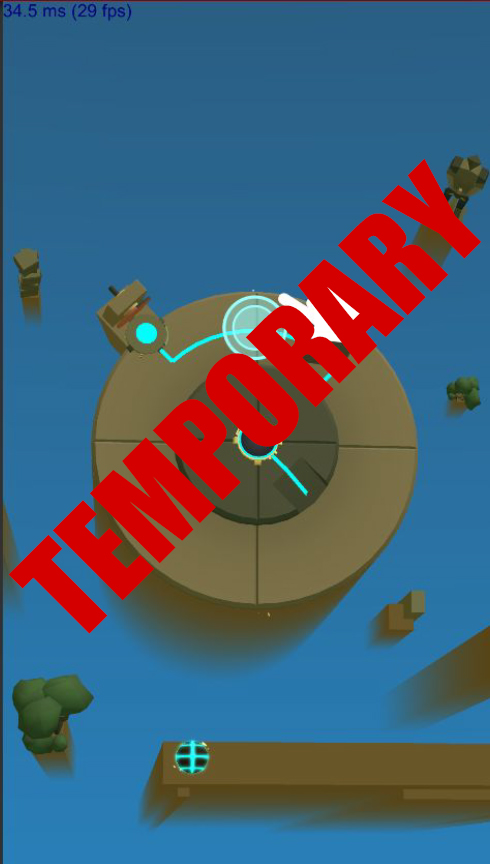
\includegraphics[height=8cm]{fig/tmp.jpg}
	\caption{Wygląd przykładowego poziomu gry \textit{Sphaze}.}
	\label{fig:sphaze_1}
\end{figure}

Osoba grająca nie ma wpływu na ruch sfer, jedynie na obrót pierścieni planszy. Każda rotacja na tych elementach powoduje zmianę połączeń między ścieżkami na nich się znajdującymi. Kule cały czas poruszają się do przodu, chyba że spotkają na swojej drodze skrzyżowanie. Wybierają wtedy ścieżkę, którą zdefiniować można jako "najbardziej prawą". Oznacza to, mając możliwość skręcenia w prawo, zawsze wybiorą tą opcję. Gdy nie ma możliwości obrotu w prawo, sprawdzane jest, czy dostępna jest ścieżka na wprost. W następnej kolejności przeprowadzony zostaje test, czy istnieje skręt w lewo. W przypadku braku możliwości wyboru żadnej z przedstawionych opcji, uznawane jest, że natrafiono na "ślepy zaułek", konieczne jest zatem zawrócenie.

Użytkownik decyduje również, z którego miejsca na planszy ma wystartować jaka sfera. Wprowadzenie pierwszej kuli na strefę labiryntu traktowane jest jako rozpoczęcie rozgrywki. Przykładowe punkty startowe, na których ustawić można kule ukazane zostały na rysunku \ref{fig:sphaze_startpoints_1}. Zauważyć można, iż znajdują się one wszystkie na obrzeżach planszy. Jest to reguła, którą gracz jest w stanie bardzo szybko zauważyć. Dzięki temu na późniejszych poziomach gracze nie próbują ich szukać w żadnym innym miejscu. Z racji na fakt, iż "rozbijają" one okrągłą sylwetkę planszy wyjątkowo łatwo je dostrzec nawet gdy gra aktualnie ich nie wyróżnia. 
Na każdym poziomie zdefiniowane jest ograniczenie czasowe, którego przekroczenie jednoznacznie wiąże się z koniecznością powtórzenia zadanej planszy. Czasomierz, którego zadaniem jest informowanie użytkownika o tym jak dobrze sobie on radzi, rozpoczyna odliczanie wraz z rozpoczęciem rozgrywki, czyli gdy pierwsza kula zacznie poruszać się w przestrzeni poziomu. 

\begin{figure}[h!]
	\centering
  	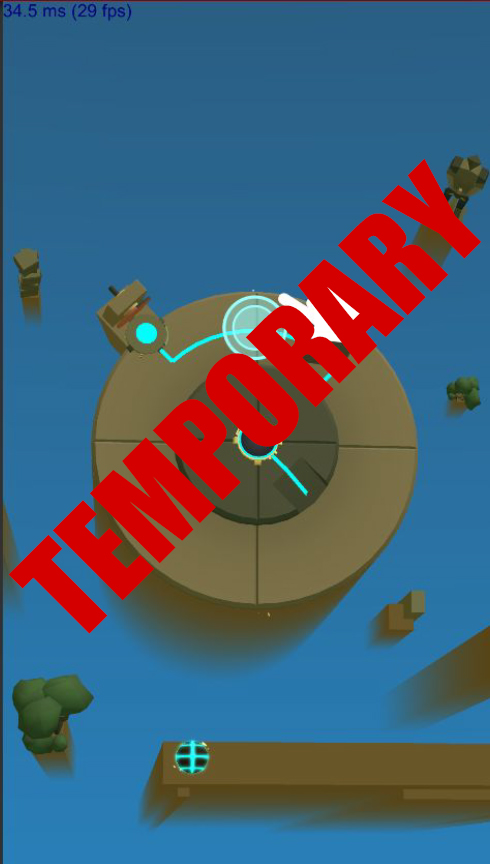
\includegraphics[height=8cm]{fig/tmp.jpg}
	\caption{Przykładowe rozmieszczenie punktów startowych na poziomie. Punkty startowe zostały oznaczone czerwonymi okręgami.}
	\label{fig:sphaze_startpoints_1}
\end{figure}

Gracz ma ograniczoną kontrolę nad rozgrywką, gdyż jego akcje wpływają jedynie pośrednio na jej przebieg. Obrót pierścieni wpływa jednie na możliwości ruchu, jakimi dysponują kule. Zadaniem użytkownika jest dostosowanie się do tego stanu i przewidzenie, jak obiekty poruszać się będą w zadanym przez niego środowisku. Nieświadome podejmowanie decyzji może bowiem prowadzić do sytuacji, które szybko potrafią stać się mało zrozumiałe dla użytkownika, który nie do końca rozumie, co się dzieje w przestrzeni gry.

	\subsection{Samouczki}
Wymagane jest zatem, by gracz przyswoił podstawowe prawa tej gry jak najszybciej. W przeciwnym wypadku spodziewać się można, iż prędko zacznie odczuwać frustrację spowodowaną pozornie małym wpływem jego akcji na finalny wynik gry. 

Z tego też powodu przygotowane zostały tzw. samouczki mające na celu wyjaśnienie użytkownikowi kluczowych mechanik. Nowe informacje przekazywane są stopniowo. Każdy kolejny element kluczowy jest najpierw przedstawiany w prostym, kontrolowanym środowisku, a następnie powtarzany już w coraz bardziej złożonych sytuacjach. 
W przeprowadzanym badaniu analizowane były trzy główne mechaniki: 
\begin{itemize}
\item sposób na startowanie rozgrywki na danym poziomie, 
\item obracanie pierścieniami,
\item ruch kulek (fakt, iż zawsze skręcają one w najbardziej prawą ścieżkę.
\end{itemize}

W celu poprawnego nauczenia tych mechanik przygotowane zostały dwa testowe poziomy. W pierwszym z nich przedstawiane są podstawowe dwie zasady gry. Akcja jaką, użytkownik ma wykonać zostaje przedstawiona wizualnie bez użycia tekstu. Sam gracz musi zrozumieć, że jego ruchem powinno być odzwierciedlenie tego, co pokazywane mu jest na ekranie. Należy zauważyć, że użytkownik nie zawsze jest w stanie również przewidzieć co się wydarzy, gdy wykona zadane mu zadanie. Dopiero po wykonaniu ukazanej akcji jest w stanie przeanalizować jaki wpływ miały jego ruchy na przestrzeń gry.
Wygląd poszczególnych etapów tego poziomu dla jednej wersji gry przedstawiony został na rysunku \ref{fig:tut_L1_1}.

\begin{figure}[h!]
	\centering
  	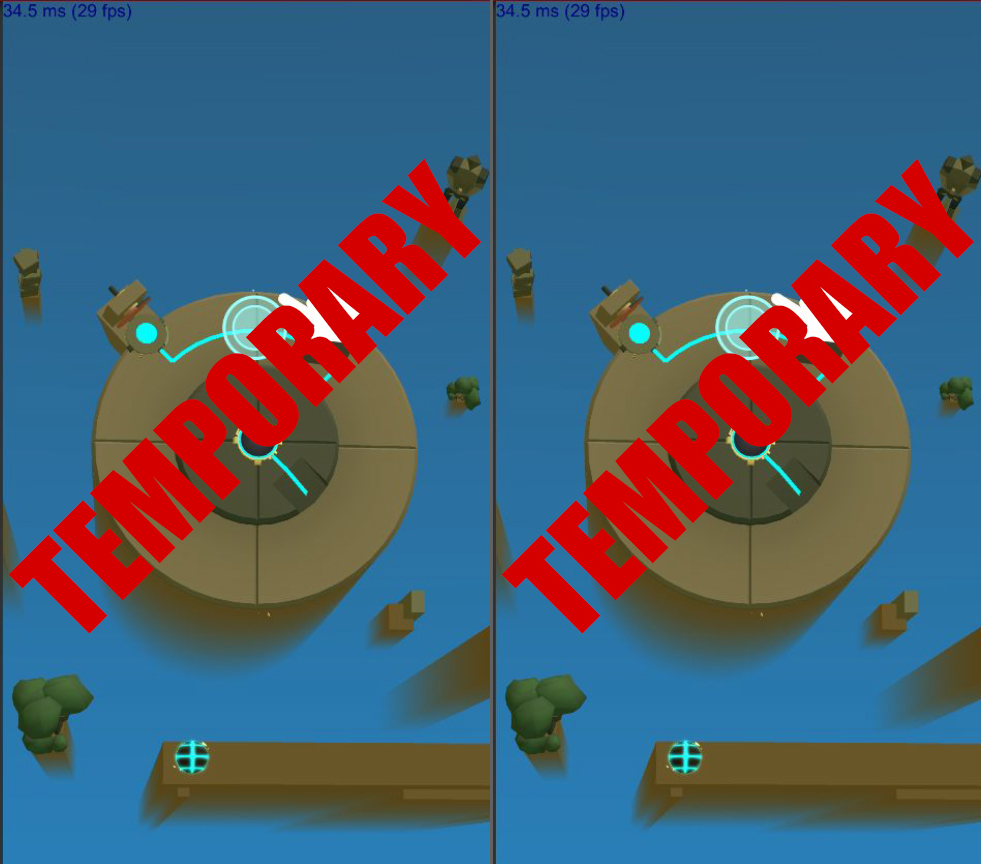
\includegraphics[height=8cm]{fig/tmp2.jpg}
	\caption{Wygląd pierwszego samouczka przed którym postawiony jest gracz.}
	\label{fig:tut_L1_1}
\end{figure}

Plansza dla tego poziomu składa się z dwóch poziomu składa się z dwóch pierścieni. Nie można poruszać pierścieniem w samym środku, co sprawia, że jedynym fragmentem labiryntu, z którym użytkownik może wchodzić w interakcję jest zewnętrzny pierścień.
Gdy gracz włączy ten poziom wymagane jest od niego aby najpierw obrócił właśnie ten element. Celem jest doprowadzenie do połączenia ścieżek znajdujących się na pierścieniach. Gdy gracz wykona ruch powodujący rozłączenie tych dróg, samouczek powróci do tego etapu. Pozwala to w łatwy sposób uzmysłowić użytkownikowi, o wadze, jaką ma stworzenie odpowiedniej drogi dla kul. 
Następnym zadaniem jest ustawienie jedynej sfery na poziomie w jej miejscu startowym. Samouczek znika dopiero w momencie poprawnego wykonania tej akcji. Gdy to nastąpi i użytkownik nie wprowadzi dalszych zmian w obrocie pierścieni, kula w szybki sposób dociera do środka labiryntu, a co za tym idzie - kończy poziom.

Drugi samouczek ustawiony został dopiero na trzeciej planszy. W tym miejscu chcemy zwrócić uwagę gracza na zachowanie kul w momencie dotarcia do skrzyżowania. Wygląd tego poziomu zobaczyć można na rysunku \ref{fig:tut_L3_1}. Labirynt w tym wypadku składa się z trzech pierścieni, z czego z dwoma z nich użytkownik może wejść w interakcję. Obecny tutaj samouczek wyzwala się dopiero w momencie, gdy za przeprowadzonymi wcześniej akcjami gracza sfera dotrze do skrzyżowania znajdującego się na środkowym pierścieniu. Zostaje wtedy zabrana użytkownikowi kontrola a kamera skupia się na problematycznym miejscu. Oprócz tego, zanim zostanie wykonany manewr kulki, zostaje pod nią narysowana strzałka wskazująca, w którą stronę ona skręci. Gry kulka opuszcza skrzyżowanie, kamera wraca do podstawowej pozycji a ruchy gracza znowu wpływają na układ pierścieni. Całość opisanych akcji zajmuje podczas normalnej gry tylko ułamek sekundy, dlatego czas gry zostaje w tym momencie czterokrotnie spowolniony. 
\begin{figure}[h!]
	\centering
  	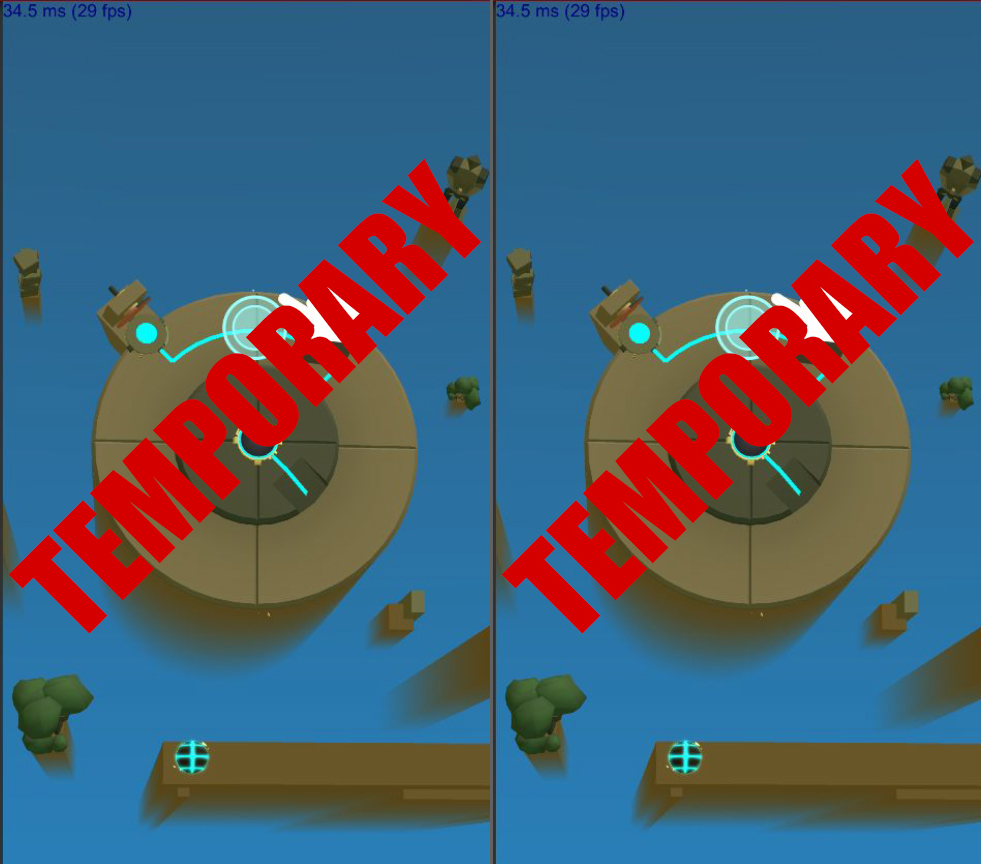
\includegraphics[height=8cm]{fig/tmp2.jpg}
	\caption{Wygląd poziomu zawierającego samouczek tyczący się skrętu kul. Czerwonym okręgiem zaznaczone zostało skrzyżowanie.}
	\label{fig:tut_L3_1}
\end{figure}
Mimo tego, całość przedstawionych operacji trwa niecałe trzy sekundy. Oprócz tego składa się z ruchów kamery, które użytkownik widzi jedyny raz w tym miejscu rozgrywki. Istnieje zatem szansa, iż nie uda mu się zrozumieć pełnego przekazu, który miał być zawarty w tym samouczku. Dlatego też następne dwa poziomy, które zobaczyć można na rysunku \ref{fig:tut_L3_2}, stworzone zostały z myślą o tym, by pomóc graczom ze zrozumieniem mechaniki skrętu kul. W obydwu tych poziomach rozwiązanie, które jest początkowo sugerowane, powoduje powstanie sytuacji, w której kulka skręcając w prawo oddala się od środka labiryntu. Użytkownicy, którzy nie rozumieją jeszcze sposobu poruszania się kulki bardzo szybko są wtedy w stanie zauważyć, że kryje się za tym jakiś algorytm. Gdy to zostanie osiągnięte, zrozumienie w jaki sposób wyznaczana jest trasa dla sfery przychodzi znacznie łatwiej.

\begin{figure}[h!]
	\centering
  	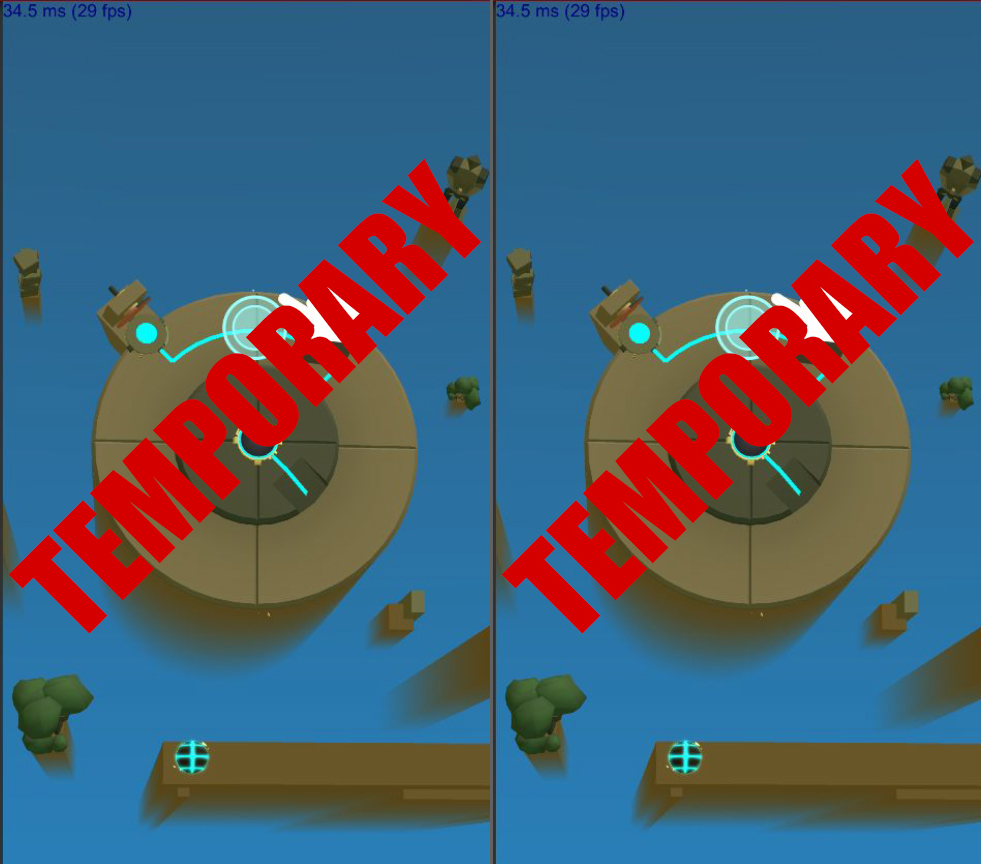
\includegraphics[height=8cm]{fig/tmp2.jpg}
	\caption{Początkowy wygląd czwartego i piątego poziomu gry \textit{Sphaze}. Mają one na celu pomóc użytkownikowi zrozumieć mechanikę ruchu kul.}
	\label{fig:tut_L3_2}
\end{figure}

\section{Heurystyki}
Z listy heurystyk PLAY \cite{ArticlePLAY} wybrane zostały dwie zaliczające się do kategorii użyteczności oraz mechanik gry. Określają one, jak projektowana powinna być gra, by grywalność była jak największa. Wyróżnione heurystyki zostały wybrane jako nietrywialne i subiektywnie najprostsze do efektywnego zweryfikowania. Opisane one zostały w tabeli \ref{tab:tab1}.

\begin{table}[h!]
  \centering
  \caption{Wybrane analizowane heurystyki PLAY z dziedziny informacji o statusie i wyniku.}
  \label{tab:tab1}
  \begin{tabular}{|r|l|}
    \hline
    1. & Wskaźniki wyniku są płynne, oczywiste, dostępne oraz nie wpływają na rozgrywkę.\\
    \hline
    2. & Sterowanie jest intuicyjne i mapowane w sposób naturalny.\\
    \hline
  \end{tabular}
\end{table}

\section{Rodzaje interfejsów}
W rozgrywce widoczny jest jedynie jeden wskaźnik statusu - określa on pozostały użytkownikowi czas na poziomie. Przedstawić go można jako jako dwuwymiarowy przycisk podobny do tego, który używany jest do zatrzymania gry, lub jako siatkę w przestrzeni gry. Każde podejście ma swoje zalety. W przypadku elementu 2D użytkownik nie ma wątpliwości co do jego informacyjnego przeznaczenia. Dla wersji w świecie gry nie zawsze to musi być spełnione. Wręcz przeciwnie, użytkownik, który dopiero uczy się na czym polegają mechaniki gry może odczuć frustrację bądź zniechęcenie wywołane tym, że nie jest możliwe wejście w interakcję z elementem umieszczonym w bezpośredniej przestrzeni gry. Plusem tego rozwiązania jest dużo bardziej zrozumiałe połączenie między fragmentami rozgrywki. Prostszym zdaje się zrozumienie powodu startowania czasomierza w chwili ustawienia pierwszej kulki na planszy, gdy zarówno labirynt, jak i reprezentacja zegara współdzielą ze sobą jedną przestrzeń.

Spełnianie drugiej z wybranych heurystyk określić można jako sterowanie zbliżone do tego, jak wyglądałoby wykonywanie akcji z gry w normalnym świecie. Tak więc, aby obrócić pierścień naturalnym zdaje się ruch przeciągania. Również przeniesienie kulki z miejsca na miejsce wydaje się oczywiste, że powinno zostać wykonane poprzez "złapanie" jej i przeciągnięcie w miejsce docelowe gdzie finalnie następuje jej "upuszczenie". Dzięki takiemu podejściu do tych mechanik uzyskane zostaje wrażenie fizyczności obiektów w przestrzeni gry. Stworzona zostaje iluzja, że zachodzi faktyczna interakcja z obiektami, które wyświetlane są na ekranie. Inaczej prezentuje się to przy mniej realnej wersji interakcji. Wykorzystana w niej zostaje inna znana mechanika z urządzeń mobilnych - proste kliknięcie w interesujące nas miejsce. Tym sposobem użytkownik jest w stanie zakomunikować, w którą stronę chce obrócić pierścień poprzez dotknięcie go z odpowiedniej strony. Przeniesienie kulki w tym scenariuszu odbywa się poprzez dotknięcie wybranej sfery, a następnie powtórzenie tej akcji dla miejsca docelowego. W tym wypadku użytkownik, który dobrze rozumie te mechaniki może znacznie szybciej wykonywać akcje w trakcie gry. Wiąże się to jednak z utratą części wiarygodności, którą uzyskać można było sposobem pierwszym.

Na podstawie wybranych heurystyk przygotowane zostały zatem cztery wersje gry. Każda z nich spełnia inną kombinację zadanych założeń. Takie podejście pozwala na dokładne przetestowanie, jaki wpływ zasady te mają na grywalność aplikacji. 
\subsection{Interfejs SWIPE 2D}
Jako pierwszy wyróżniony został interfejs \textit{SWIPE 2D}, który w założeniu spełnia zarówno pierwszą, jak i drugą heurystykę. Jego reprezentację graficzną dla pierwszego poziomu gry zobaczyć można na rysunku \ref{fig:interface_swipe_2d}. Zegar zdefiniowany jest w nim jako element dwuwymiarowy znajdujący się w górnej części ekranu, a wszelkie interakcje rozwiązane są poprzez jak najwierniejsze odwzorowanie ich odpowiedników z rzeczywistości. Spodziewać się zatem można najmniejszej ilości błędów popełnianych przez użytkowników już od samego początku gry. Również różnice w czasach pojedynczego testu powinny być dla tej wersji względnie niewielkie.
\begin{figure}[h!]
	\centering
  	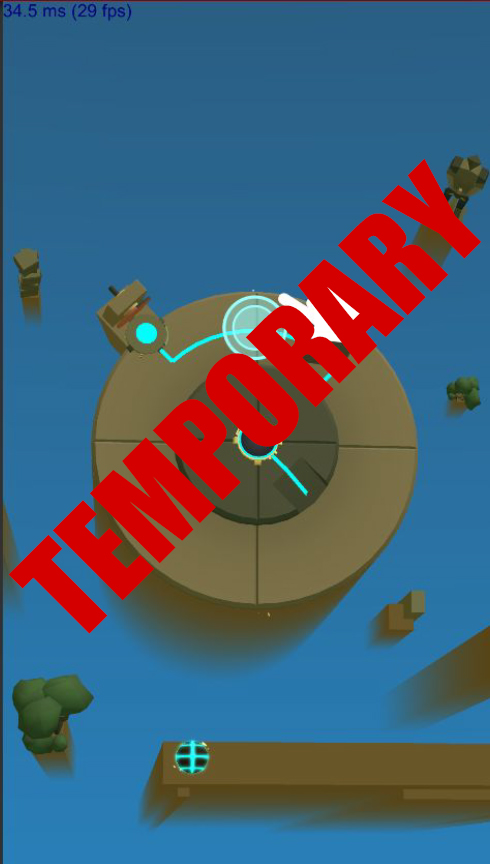
\includegraphics[height=8cm]{fig/tmp.jpg}
	\caption{Wygląd poziomu pierwszego dla wersji gry wykorzystującej interfejs \textit{SWIPE 2D}.}
	\label{fig:interface_swipe_2d}
\end{figure}
\subsection{Interfejs SWIPE 3D}
Wersja interfejsu wykorzystująca mechanikę przesuwania lecz niespełniająca pierwszej z wybranych heurystyk określona została mianem \textit{SWIPE 3D}. Jego wygląd zaprezentowany jest na rysunku \ref{fig:interface_swipe_3d}. Siatka stanowiąca zegar umieszczona została w świecie gry, jako element znajdujący się wizualnie przy wyborze kul. Położenie to zostało zmienione z racji na charakterystyczne ustawienie kamery w grze. Nie pozwala ono na ustawienie tak ciężkiego elementu powyżej labiryntu, gdyż wpływałoby to negatywnie na estetykę gry. To rozwiązanie wpływać może rozgrywkę, gdyż niewykluczona jest sytuacja, w której gracz może odbierać czasomierz jako element, z którym  należy wejść w jakąś interakcję. Spodziewać się tu można zatem większej ilości błędów, które popełniane mogą być przy pierwszej styczności użytkownika z grą.
\begin{figure}[h!]
	\centering
  	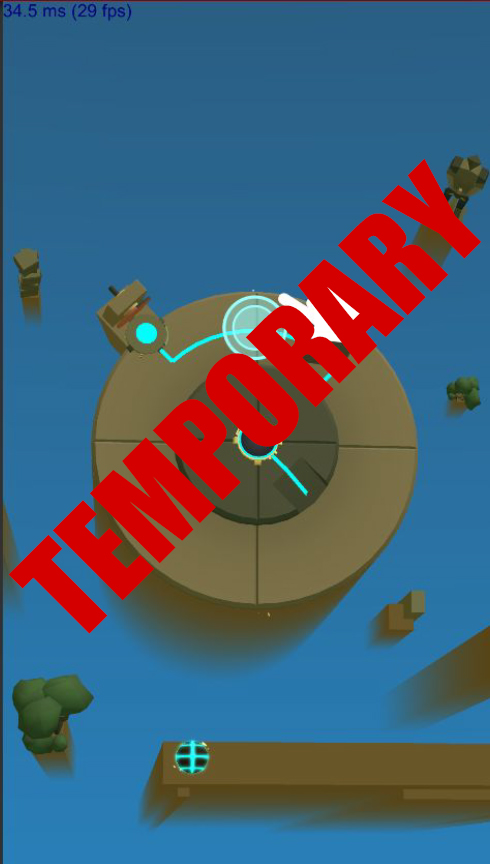
\includegraphics[height=8cm]{fig/tmp.jpg}
	\caption{Wygląd poziomu pierwszego dla wersji gry wykorzystującej interfejs \textit{SWIPE 3D}.}
	\label{fig:interface_swipe_3d}
\end{figure}
\subsection{Interfejs CLICK 2D}
Interfejs \textit{CLICK 2D} wizualnie nie rózni się od wersji \textit{SWIPE 2D}. Zmieniony jest tu jednak styl sterowania głównymi mechanikami gry na takie, które są w znacznie mniejszym stopniu reprezentacją rzeczywistych interakcji. Cechują się one tym, że by osiągnąć ten sam cel wykonywane mogą być znacznie szybsze ruchy (kliknięcie zamiast przesuwania palca po ekranie). Oznaczać to może, że doświadczony użytkownik jest w stanie uzyskać w tej wersji lepsze czasy niż ten, który umiejętnie posługuje się wersją z mechaniką przesuwania. Idąc tym tropem założyć można, iż różnica w czasach przechodzenia poszczególnych poziomów będzie zatem tutaj zauważalnie większa, gdyż wymaga on nauczenia się mniej intuicyjnej zasady gry.
\subsection{Interfejs CLICK 3D}
Podobnie jak w poprzednim przypadku, w wersji interfejsu \textit{CLICK 2D} brak jest różnic wizualnych względem \textit{SWIPE 2D}. W tym wypadku jednak nie jest spełniona żadna ze sprawdzanych heurystyk. Oznaczać to może, że wyniki dla tego wypadku będą najmniej korzystne. Spodziewać się można dużej ilości początkowych błędów spowodowanych mniej odciętym od całości gry zegarem oraz większych różnic w statystykach podczas przechodzenia tego samego poziomu dwukrotnie przez pojedynczego gracza.
\section{Struktura badania}
Na potrzeby przeprowadzenia testów przygotowane zostało badanie mające na celu wydobycie z przebiegów gry przydatnych informacji. 
Użytkownik miał za zadanie zagrać w przygotowaną wcześniej grę w ściśle określony sposób:
\begin{itemize}
\item przejść pierwszych pięć poziomów,
\item zagrać w arbitralnie dobraną liczbę następnych plansz (przynajmniej 5),
\item ponownie rozegrać pierwszych pięć poziomów.
\end{itemize}
Zarówno przed jak i po przeprowadzeniu badania osoba testująca nie musiała wypełniać żadnej ankiety odnośnie swoich wrażeń z gry. Oznacza to też, iż dane takie jak płeć, czy wiek gracza nie były brane pod uwagę w dalszej ocenie wyników. Gra automatycznie zapisywała wyniki badania do pliku, który później podlegał analizie.

Zauważyć należy iż dane zbierane były tylko dla pierwszych pięciu plansz. Powtórzenie ich przejścia na koniec indywidualnego testu jest kluczowe dla wyników badań. Przy pierwszym podejściu do poziomów 1-5 gracz nie wie, czego aplikacja może od niego wymagać. Jest to jego pierwsze starcie z mechanikami, których musi się nauczyć. \
Inaczej sprawa się ma z drugimi wynikami danej osoby badanej. Z racji tego, że wymagane jest by przeszła ona przynajmniej 10 poziomów, założyć można, iż zaznajomiła się ona z podstawowymi prawami gry. Różnice pomiędzy tymi wynikami pozwalają na określenie jak dużego postępu dokonał gracz, o ile lepiej zrozumiał zadane mechaniki. Zminimalizowana zostaje w ten sposób różnica pomiędzy umiejętnościami różnych osób. Gdy porównywane są one do samych siebie nie nie trzeba brać pod uwagę czynników, takich jak przykładowo predyspozycje do sprawnego przechodzenia gier logicznych.

Pomijalny staje się również wpływ, jaki miało środowisko, w którym przeprowadzany był eksperyment. W uproszczeniu założyć można, że w warunkach, jakie były zapewnione użytkownikom zarówno oświetlenie, jak i poziom hałasu utrzymywał się na jednym poziomie dla jednego testu.

Same testy odbywały się zarówno na wyciszonym, względnie odizolowanym pomieszczeniu ale także w dużo trudniejszych warunkach - jako część większych wydarzeń, bądź podczas jazdy komunikacją miejską. 

Do celów badania przygotowane zostały cztery wersje gry, które zawierały w sobie opisane wcześniej interfejsy. Osobie badanej przyznawana była losowo wybrana aplikacja z tej puli i przedstawiana była jako jedyna wersja gry. 
Badane były osoby, które nigdy wcześniej nie spotkały się z grą będącą obiektem testów. Miały one za zadanie przejść zadane poziomy bez żadnej wcześniejszej informacji o tym, jaki jest chociażby warunek przejścia do następnej planszy. Informacja o tym, że wyniki podlegają zapisowi przekazywana była dopiero wtedy, gdy wymagane było, by osoba testowana przystąpiła ponownie do pierwszych pięciu poziomów. Miało to na celu możliwe zminimalizowanie presji czasu, która mogłaby się pojawić przy otrzymaniu aplikacji do testowania.(JAKIŚ LINK?)

Dla każdego przejścia poziomu przez danego użytkownika zebrane zostały następujące dane:
\begin{itemize}
\item czas absolutny, 
\item czas ruchu kuli,
\item ilość obrotów pierścieni,
\item ilość dotknięć ekranu.
\end{itemize}
Oprócz tego, obliczona została dodatkowa zmienna, która zależna jest od czasu absolutnego oraz czasu ruchu kuli - czas myślenia użytkownika.

	\subsection{Czas absolutny}
Czas, który użytkownik potrzebował na przejście poziomu, licząc od jego załadowania określany jest mianem absolutnego $t_{abs}$. Zawiera on w sobie długość trwania obejrzanej przez użytkownika animacji wejścia poziomu, a jego liczenie przerywane jest wraz z wejściem ostatniej kuli na poziomie do środka labiryntu. Czas ten nie zawiera zatem w sobie informacji o tym, jak długo użytkownik pozostawał na ekranie podsumowującym dany poziom. Spowodowane to było obserwacją, że czas spędzony w tym ekranie uznany został za pomijalny w przeprowadzanych badaniach.
	\subsection{Czas kuli}
Oprócz obliczania tego, ile czasu potrzebne było użytkownikowi na przejście poziomu wymiernym okazało się również sprawdzanie jak optymalne ścieżki wybrane zostały dla sfer. Wszystkie plansze, które wykorzystane zostały w badaniu korzystały tylko z jednej kulki, która na każdej z nich poruszała się z tą samą szybkością. Oznacza to, że droga ta jest wprost proporcjonalna do czasu, w jakim poruszała się kulka - $t_{ball}$. Jego obliczanie zaczyna się wraz z wykonaniem przez użytkownika akcji startu sfery w wybranym punkcie startowym labiryntu, a kończy się, podobnie jak w przypadku $t_{abs}$, wraz z dotarciem tej sfery do środka. Im większa ta zmienna, tym bardziej można przypuszczać, iż użytkownik nie przewidział, jak zachowa się kula na planszy. Zaobserwować można tutaj, w zależności od urządzenia na którym przeprowadzone zostały pomiary, iż zmienna ta jest obciążona błędem pomiaru rzędu $5 ms$.
	\subsection{Czas myślenia}
Przydatnym w celach analizy wyników okazał się również czas myślenia - $t_{think}$. Opisać go można zależnością $t_{think} = t_{abs} - t_{ball}$. Określa on, jak długo zajęło użytkownikowi opracowanie, w jaki sposób powinien podejść do przejścia poziomu. Wyekstrahowanie go z pozostałych dwóch czasów pozwoliło w prosty sposób porównywać stosunek czasu poświęconego na planowanie do tego, jaki zajęło wprowadzanie tego planu w życie przez danego użytkownika.
	\subsection{Ilość obrotów}
Jednym z kluczowych aspektów gry testowej są pierścienie, z których składają się labirynty na poziomach. Można je obracać zarówno przed rozpoczęciem ruchu kulek, jak i w jego trakcie. Dla każdego poziomu zdefiniowana jest minimalna ilość obrotów konieczna do jego przejścia ($r_{rotMin}$). W trakcie rozgrywki zliczana jest ich ilość, jakie wykonał użytkownik i oznaczana jako $r_{rot}$. 

Częsta sytuacja, gdy $r_{rot} > r_{rotMin}$  może zatem być wyznacznikiem tego, iż użytkownik nie przewidział jakiejś sytuacji, która pojawiła się w rozgrywce i musiał improwizować podczas, gdy czasomierz odmierzał już ilość sekund pozostałych do końca poziomu. Innym wyjaśnieniem znacznej ilości obrotów pierścieni na poziomie może również być fakt, iż gracz mógł zechcieć przed rozpoczęciem faktycznej rozgrywki wizualnie zobaczyć interesujące go kombinacje obrotów i opracować plan działania. Rozróżnić można, z którą sytuacją mamy do czynienia poprzez porównanie relacji czasów $t_{think}$ oraz $t_{ball}$ do tych wyznaczonych poprzez ich odpowiedniki referencyjne - $t_{thinkMin}$ i $t_{ballMin}$.
	\subsection{Ilość dotknięć ekranu}
Zliczane również jest każde dotknięcie ekranu, jakie wykonał użytkownik podczas rozgrywki (oznaczane jako $c_{scr}$). Po ich stosunku względem ilości obrotów pierścieni wywnioskować można, jak dobrze użytkownik rozumiał, jakie operacje musi wykonać, by przejść poziom. Gdy $\frac{c_{scr}}{r_{rot}} >> 1$ oznacza to, że mechaniki obrotu pierścieni i startowania kulki nie są dla użytkownika intuicyjne, popełnia przy nich błędy. Innym wytłumaczeniem może być również niezrozumienie szaty graficznej aplikacji, a co za tym idzie zgadywanie, z którymi elementami gry można wchodzić w interakcję. Liczbę wszystkich błędów dotknięć, jakie użytkownik popełnił w trakcie przechodzenia danego poziomu obliczyć można z następującego wzoru:
\begin{equation}
c_{err} = c_{scr} - r_{rot} - c_{start},
\end{equation}
gdzie  $c_{start}$ oznacza liczbę kliknięć potrzebnych do wystartowania jednej kulki w danej wersji gry. Dla interfejsów wykorzystujących mechanikę \textit{swipe} jest to $c_{start} = 1$, podczas gdy dla interfejsów typu \textit{click} wynosi ono $c_{start} = 2$.

%CHAPTER________________________________________________________________________________________WYNIKI______
\chapter{Wyniki}
Tu przedstawiam wyniki badań\\

ILU UŻYTKOWNIKÓW ZOSTAŁO ZBADANYCH, W JAKIM PRZEDZIALE\\
JAKA SPECYFIKACJA TELEFONU \\
JAKI TYPOWY CZAS BADANIA \\


DANE:\\
wykres błędów w zależności od poziomu\\



\section{Interfejs SWIPE 3D}
Tekst
\section{Interfejs SWIPE 2D}
Tekst
\section{Interfejs CLICK 3D}
Tekst
\section{Interfejs CLICK 2D}
Tekst

%CHAPTER___________________________________________________________________________________________________
\chapter{Podsumowanie i wnioski}

Popełnione błędy: 
- przez długi czas mierzone były złe dane

Co możnaby lepiej:
- experts review
- eyetracking
Wnioski:
- Poziom 3 zabiera kontrolę i to się graczom nie podobało. Układ poziomu wpływa na to, że gracze szukają tam "podstępu".

\pagenumbering{gobble}
\bibliography{biblio} 
\bibliographystyle{ieeetr}
\renewcommand{\listoffigures}{\begingroup
\tocchapter
\tocfile{\listfigurename}{lof}
\endgroup}
\listoffigures
\chapter{Zawartość płyty}
\begin{enumerate}[label={[\arabic*]}]
  \item Tekst pracy w formacie PDF
  \item Pliki z wynikami przeprowadzonych badań
  \item Plik z wynikami przeprowadzonej analizy
\end{enumerate}

%TODO: Bibliografia
\end{document}
